% ###########################################################################
\section{Experimental Setup }
\label{sec:exp_setup}
% ###########################################################################
This section describes the experimental setup and presents the results comparing
the Linux implementations of TCP and MPTCP for transporting web traffic. We
evaluated the performance of each protocol through emulations, identifying the impact of various network
parameters in both homogeneous and heterogeneous scenarios. 

For the emulations, we use the Common Open Research Emulator (CORE)~\cite{CORE}. The setup consists of
two end-hosts, one acting as a mobile device equipped with two interfaces and the other as a web server. To reach the
server, each interface of the mobile client is connected to an (emulated) access network of the corresponding technology.

To evaluate the effect of having both homogeneous and heterogeneous network access we performed 3 sets
of experiments where the interfaces used a combination of WLAN and 3G access (i.e., WLAN-WLAN, WLAN-3G, 3G-3G).
The capacity of the WLAN was randomly chosen in the range 20-30Mbps, whereas for 3G we use values in the range of 3-5Mbps.
The propagation delays are choosen in the range of 20-25ms and 65-75ms for WLAN and 3G, respectively. To be realistic
we consider a random loss of $1-2\%$ in the WLAN access.

For each experiment, the server stores a small set of files from three different classes
of websites: Wikipedia, Amazon and Huffpost. Each website contains different number of objects of different sizes.
Of the three, Wikipedia was the smallest ($15$ objects, $72$Kb total size) followed by Amazon ($54$ objects, $1$Mb total size)
and then Huffpost ($138$ objects, $3.9$Mb total size). The sites were then requested and downloaded from the mobile
client using six concurrent connections each using TCP or MPTCP, in respective experiments.


There is a significant impact of the congestion level on the behavior of congestion control protocols~\cite{ha-background-traffic-comnet-2007}.
We therefore conduct experiments both without and with background traffic.  The background traffic is a mix of TCP and UDP flows constituting one
long TCP flow and 4 UDP flows. The aggregate usage of background flows maintained at 10\% of the bottleneck link capacity to be more realistic.
The UDP flows carry data at 500kbps each in the WLAN-WLAN scenario and 100kbps each in the 3G-3G scenario.  In each run, the background flows
start before the foreground experimental traffic and end after the experimental traffic.



We define the user experience of web browsing as the time needed to download a web page, hence, we measure the average flow completion
time for each class of web page.











% ###########################################################################
\section{Experimental Results }
\label{sec:exp_results}
% ###########################################################################






\begin{figure*}
  \centering
  \begin{tabular}{ccc}
  \subfloat[Wikipedia download, $15$ objects, $72$Kb total size.\label{fig:web:wikipedia}]{
   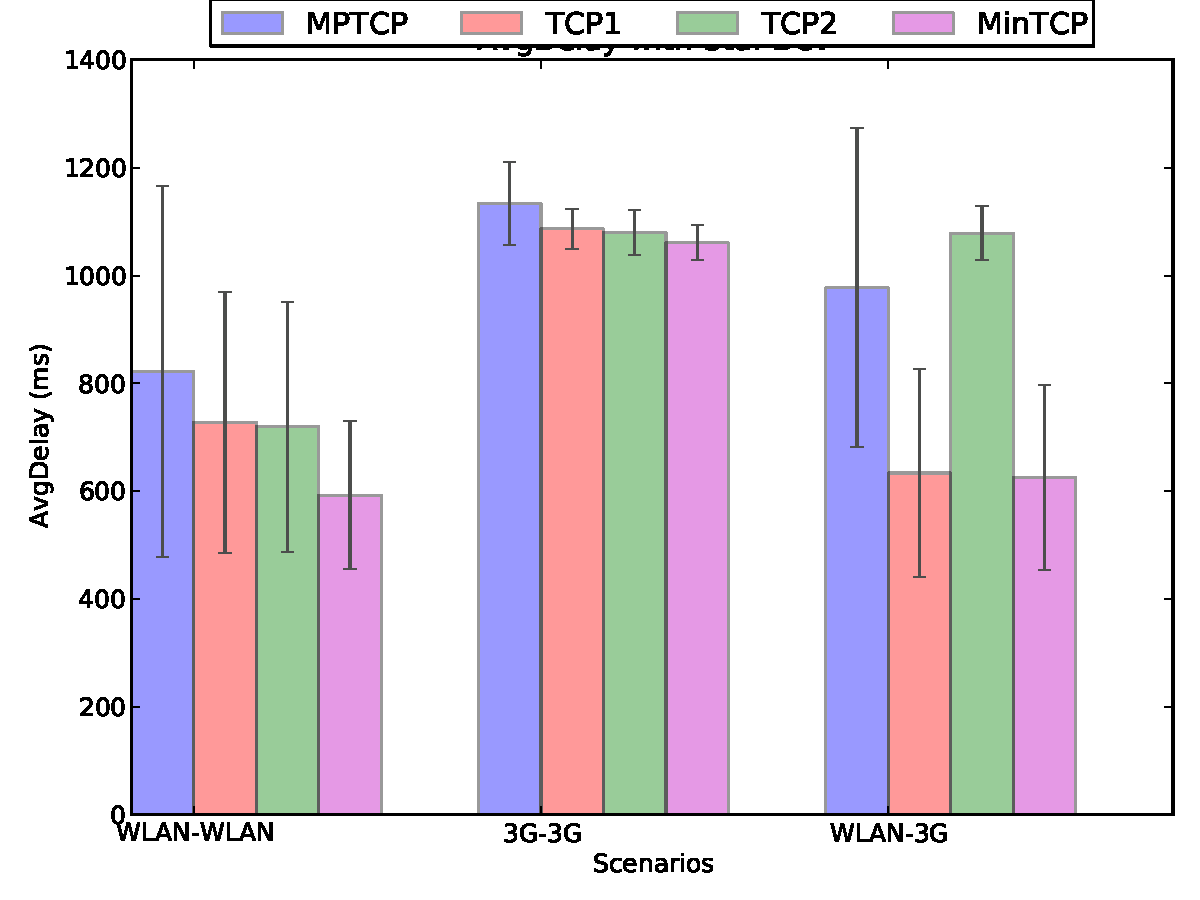
\includegraphics[width=.28\linewidth]{plots/Wikipedia_avgDelay_bar}
  } &
  \subfloat[Amazon download, $54$ objects, $1$Mb total size.\label{fig:web:amazon}]
  {
    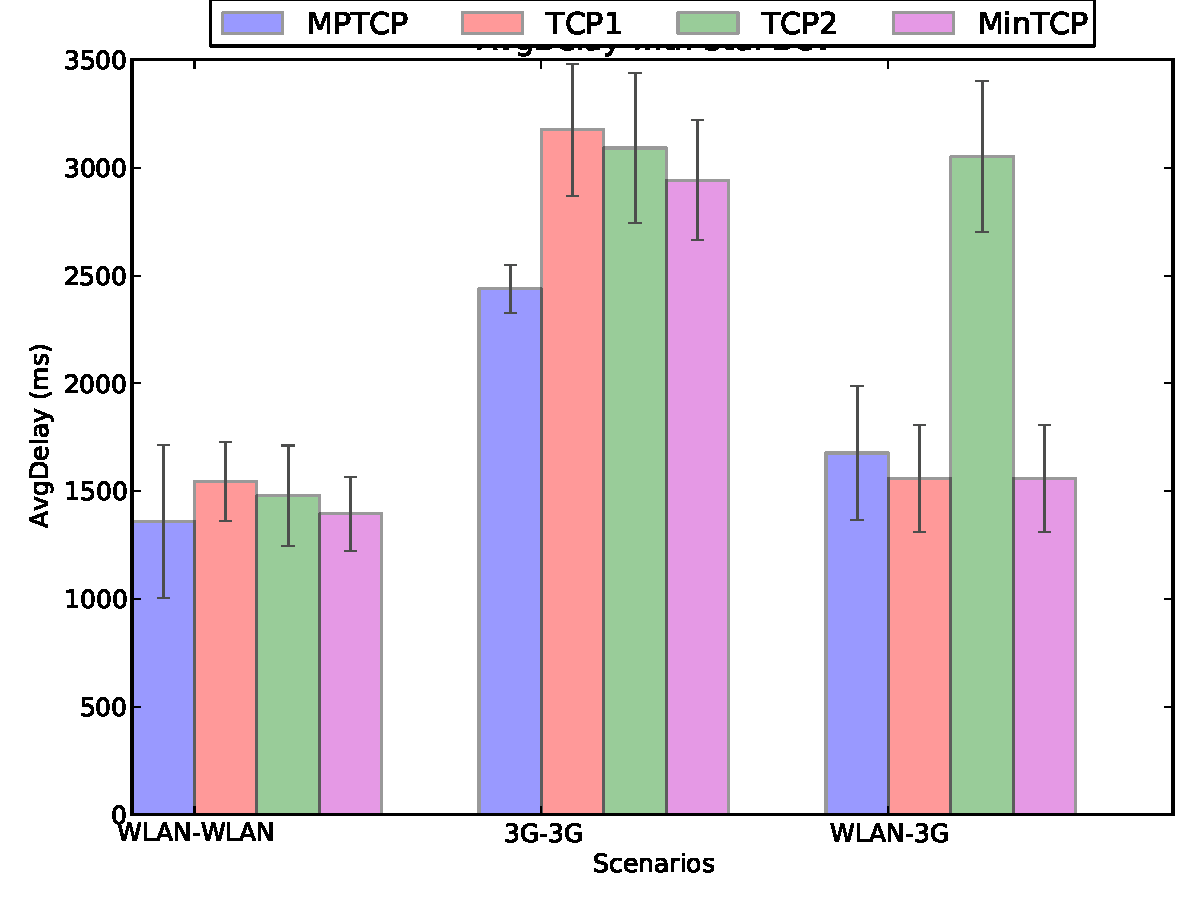
\includegraphics[width=.28\linewidth]{plots/Amazon_avgDelay_bar}
  } &
  \subfloat[Huffington Post download, $134$ objects, $3.9$Mb total size.\label{fig:web:huffpost}]
  {
    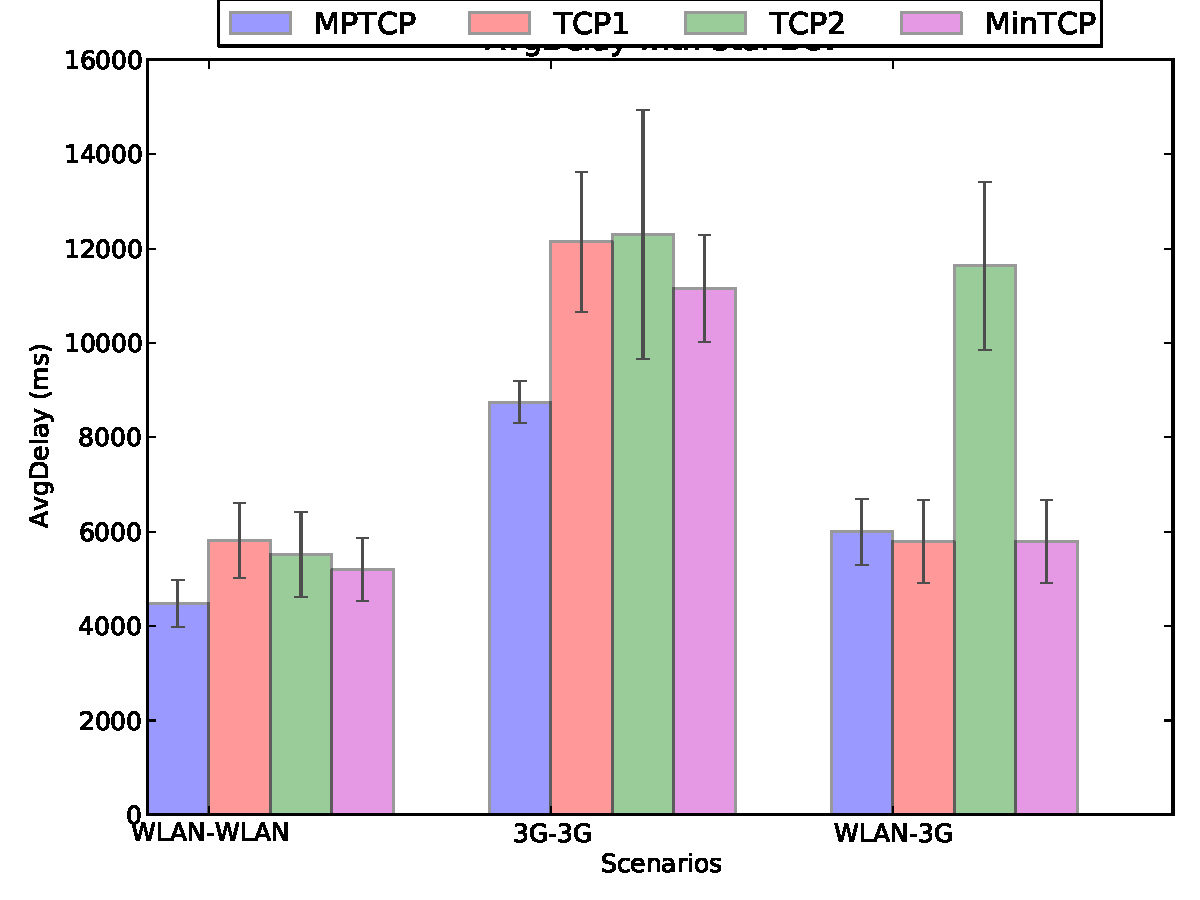
\includegraphics[width=.28\linewidth]{plots/Huffpost_avgDelay_bar}
  } 
%  \\
%  \subfloat[Wikipedia download, XYZ objects of average size XYZKB.\label{fig:web:wikipediawbg}]{
%	  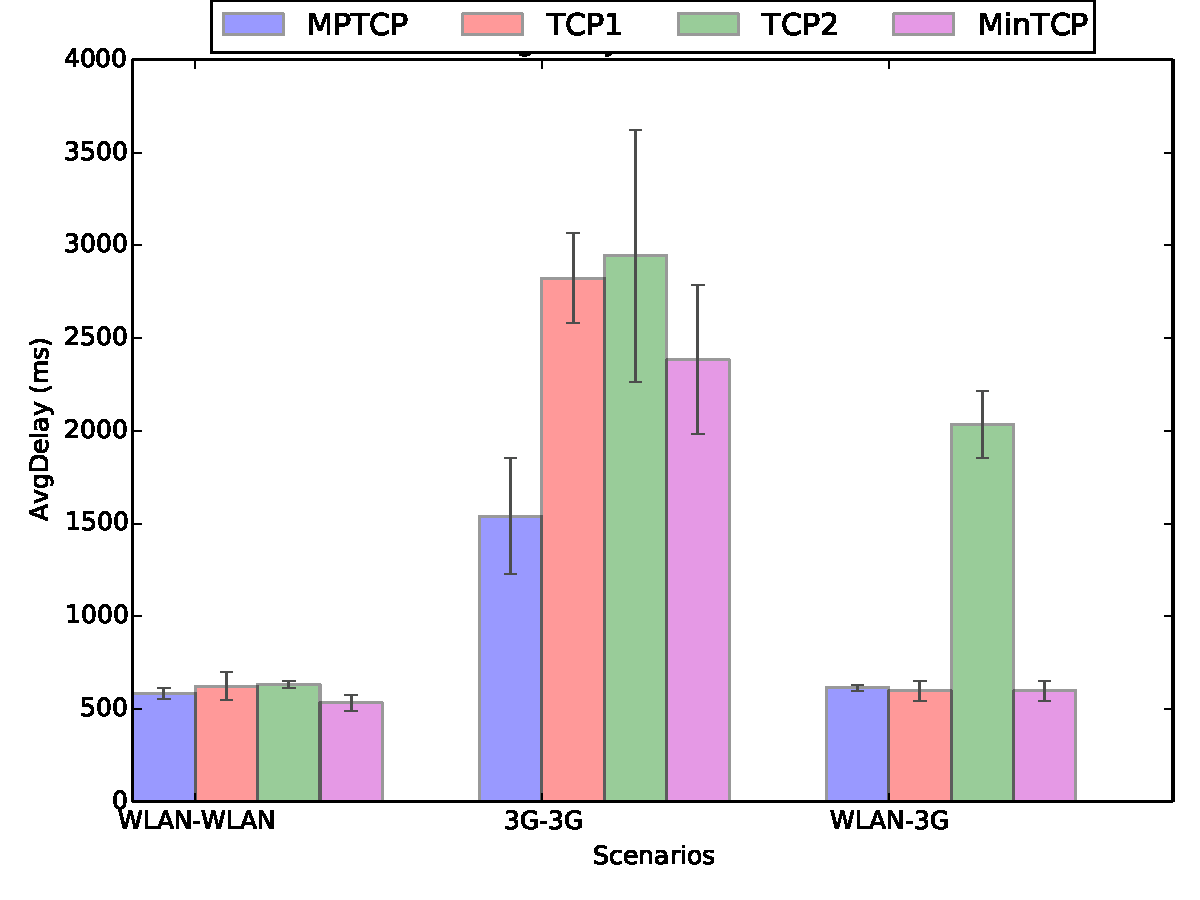
\includegraphics[width=.32\linewidth]{plots/wikipedia_avgDelayWBG}
%  } &
%  \subfloat[Amazon download, XYZ objects of average size XYZKB.\label{fig:web:amazonwbg}]
%  {
%    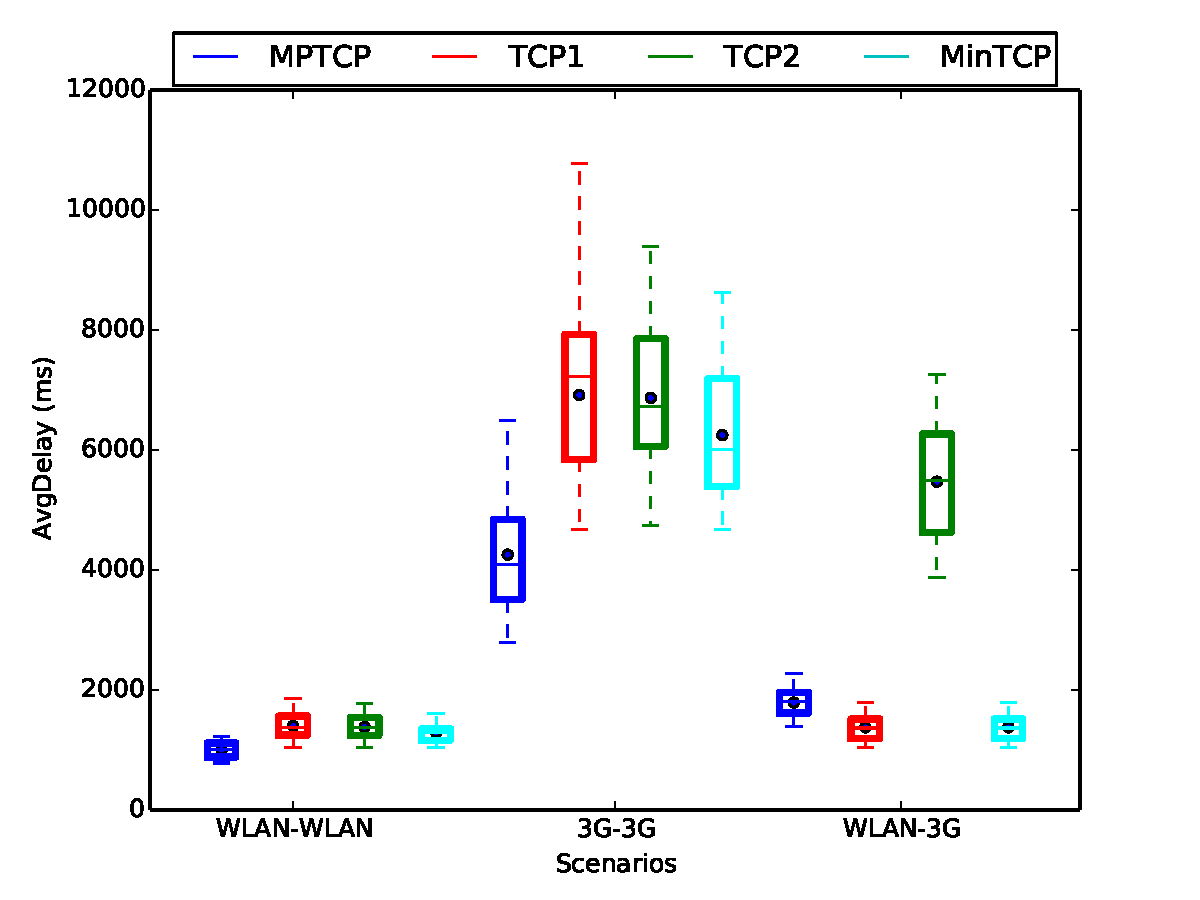
\includegraphics[width=.32\linewidth]{plots/Amazon_avgDelayWBG}
%  } &
%  \subfloat[Huffington Post download, XYZ objects of average size XYZKB.\label{fig:web:huffpostwbg}]
%  {
%    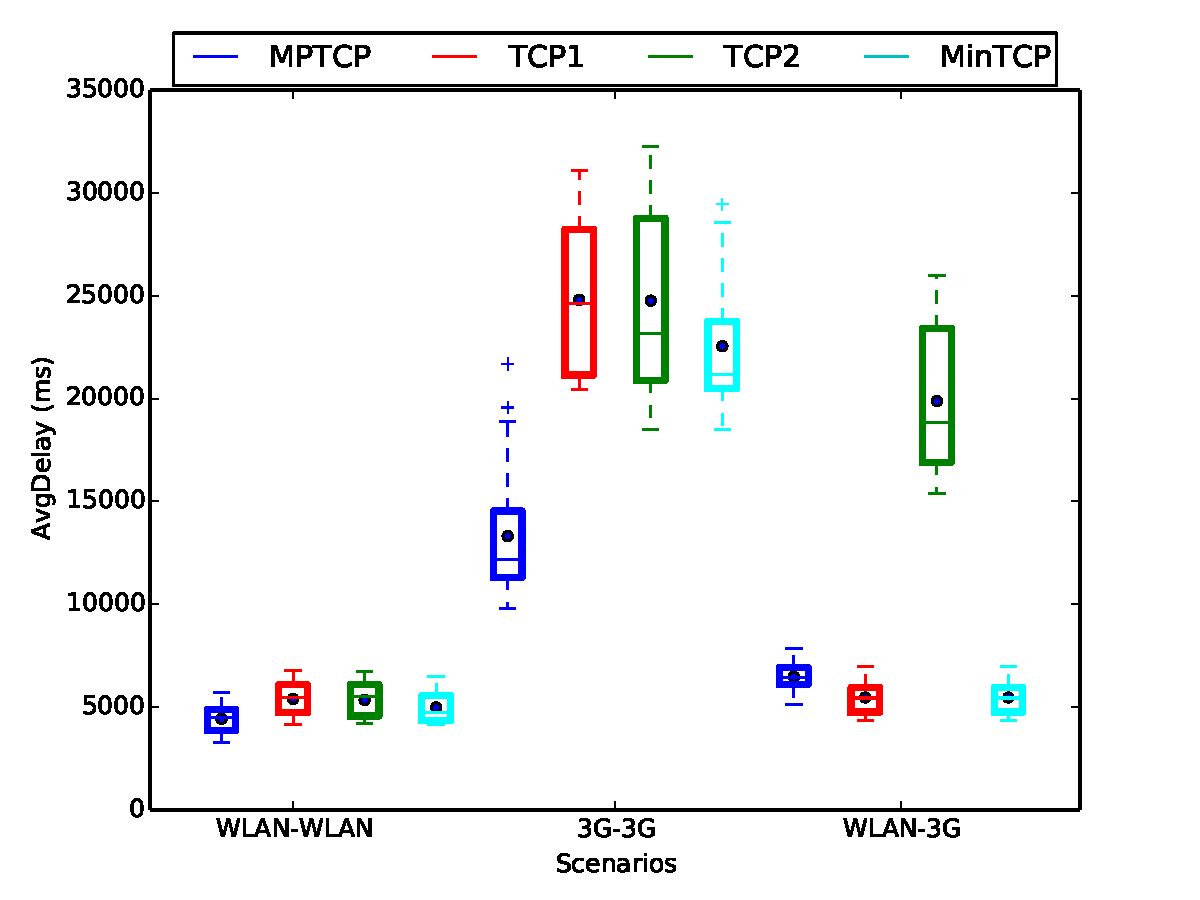
\includegraphics[width=.32\linewidth]{plots/huffpost_avgDelayWBG}
%  }
  \end{tabular}
  \caption{Average web transfer delay, with standard deviation.}
  \label{fig:web}
\end{figure*}


\begin{figure*}
  \centering
  \begin{tabular}{ccc}
  \subfloat[Wikipedia download, $15$ objects, $72$Kb total size.\label{fig:web:wikipedia-bg}]{
   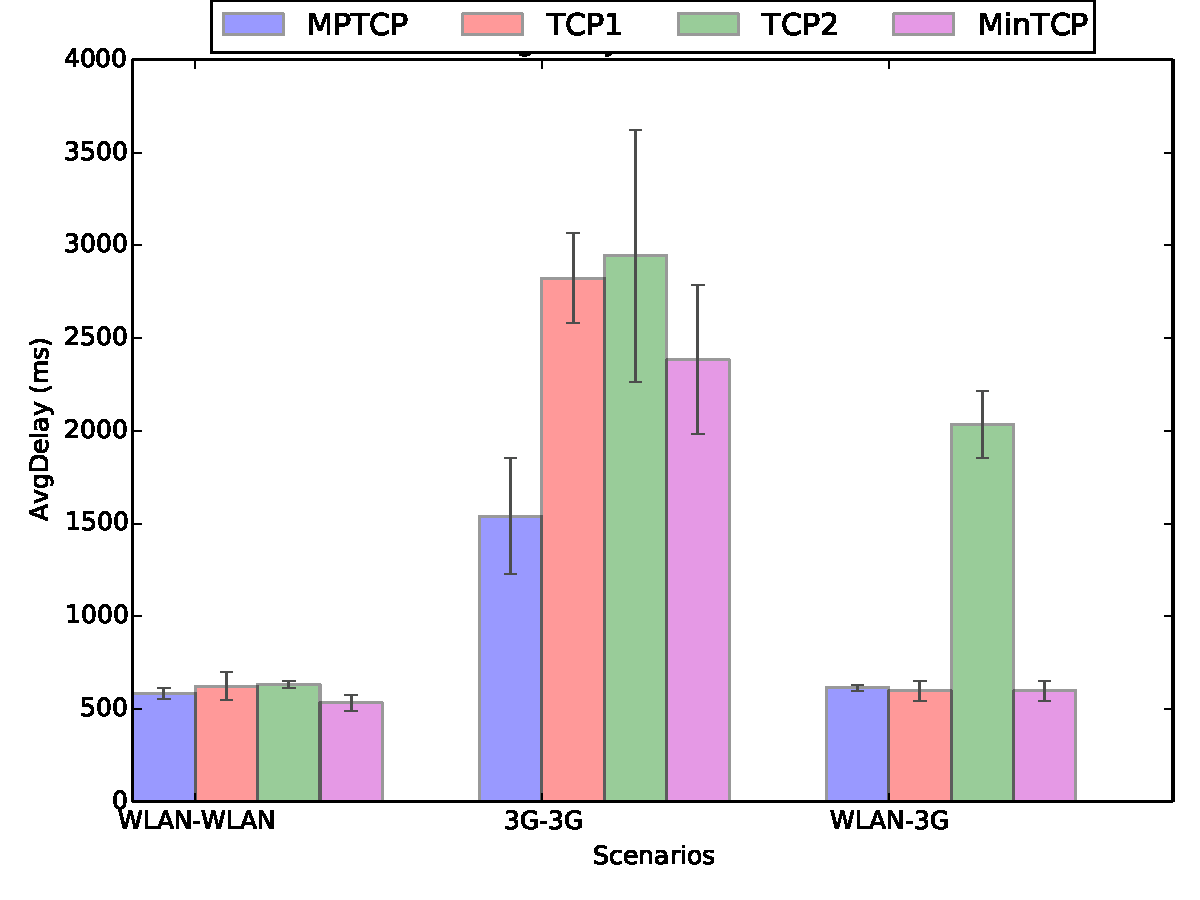
\includegraphics[width=.28\linewidth]{plots/wikipedia_avgDelayWBG}
  } &
  \subfloat[Amazon download, $54$ objects, $1$Mb total size.\label{fig:web:amazon-bg}]
  {
    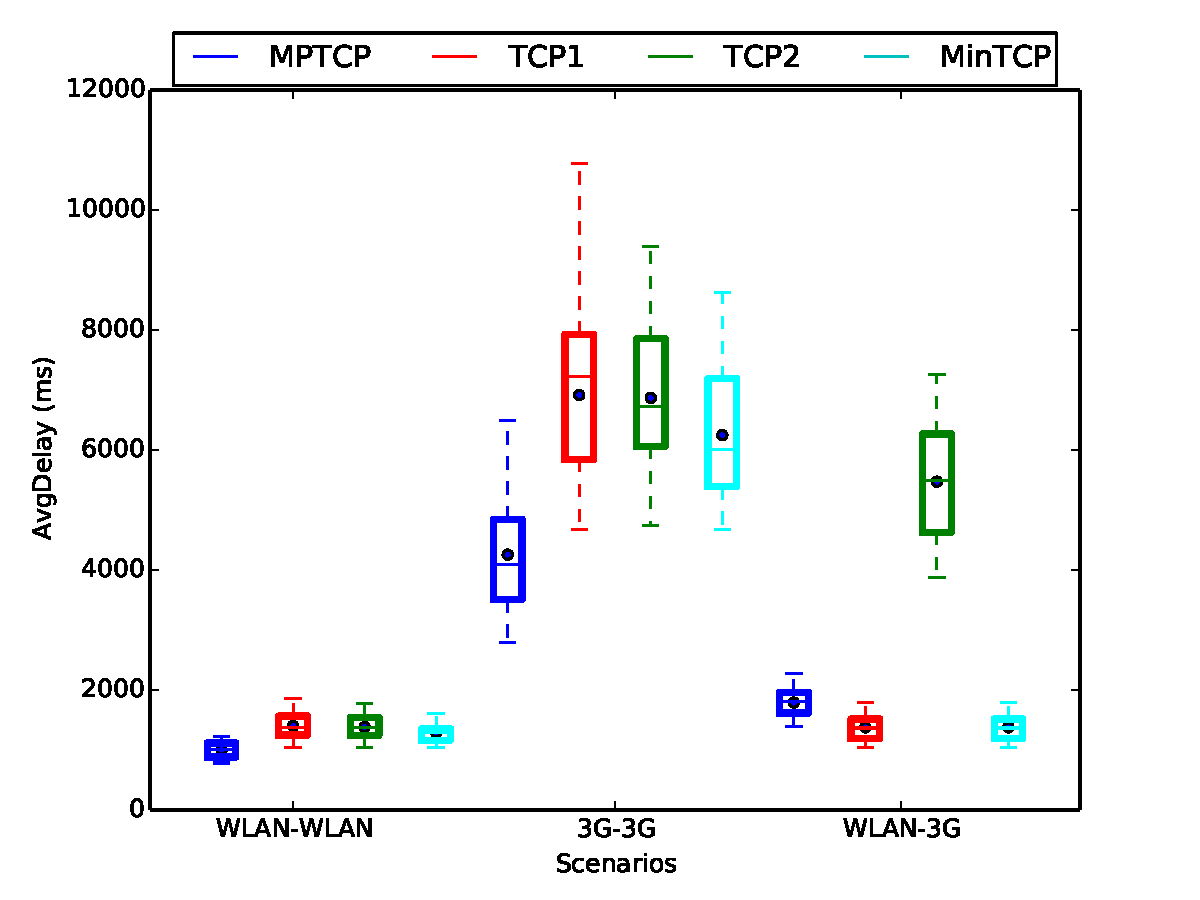
\includegraphics[width=.28\linewidth]{plots/Amazon_avgDelayWBG}
  } &
  \subfloat[Huffington Post download, $134$ objects, $3.9$Mb total size.\label{fig:web:huffpost-bg}]
  {
    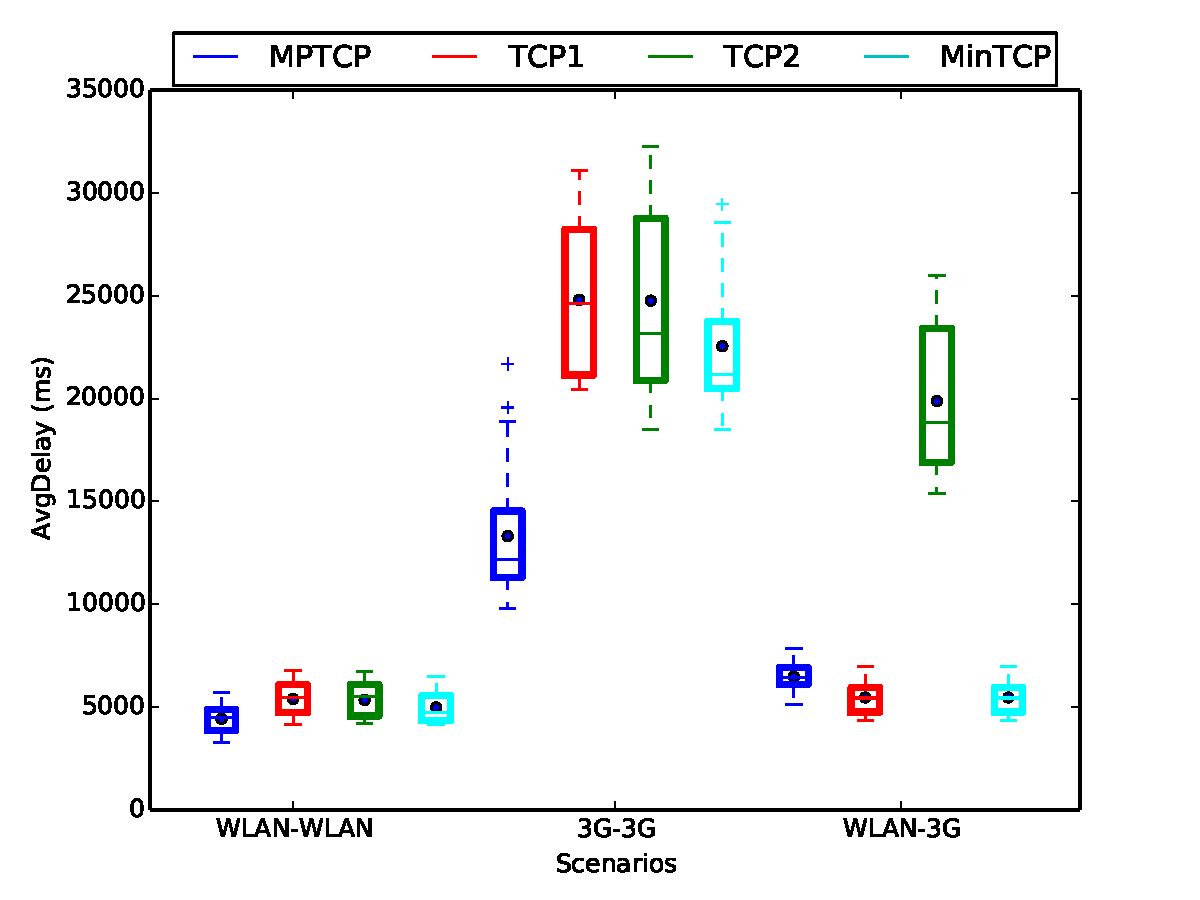
\includegraphics[width=.28\linewidth]{plots/huffpost_avgDelayWBG}
  }
 \end{tabular}
  \caption{With background flows: Average web transfer delay, with standard deviation.}
  \label{fig:web-bg}
\end{figure*}



Figure~\ref{fig:web} shows the average transfer times for web traffic, with standard variation over $30$ repetitions for 
each configuration without background traffic. Each figure depicts the average transfer time when using MPTCP, 
TCP on one of the interfaces (TCP1, TCP2), or TCP on the best available interface (MinTCP); the results are grouped according
to the emulated access networks used (WLAN-WLAN/3G-3G/WLAN-3G). We observe that MPTCP cannot reduce transfer times for the Wikipedia site, 
but is able to do so for both Amazon and Huffpost (especially in the 3G-3G scenarios). The reason for the poor performance of retrieving 
the Wikipedia site is simply that the amount of data is so small that it can be transmitted within TCP's initial window (given the six 
concurrent connections used). Employing more paths in such scenarios is not useful as long as the path itself can sustain the traffic load. 
However, for the other sites the amount of data is much larger and the transfer time can be reduced by MPTCP's implicit load-balancing over 
its available subflows; the positive effects of this load-balancing peek when the path characteristics of the subflows are homogeneous, as 
possible head-of-line blocking effects are less prevalent.


Figure \ref{fig:web-bg} illustrates the average transfer times for web traffic for emulations conducted with background traffic. 
For Wikipedia, with background traffic the results show similar behavior in the symmetric scenarios (WLAN-WLAN,3G-3G) as that of the 
no background case. In the asymmetric scenario (WLAN-3G) the performance of MPTCP is not significantly lower than that of the TCP as
seen in no background case. We observed two different aspects that could be reason for this improvement. Primarily there were losses 
in the background flows that make the background TCP flow to back off at times. We also observed that data split between the two interfaces is
not even, and more than 99\% of data transferred on the WLAN interface resulting in lower head of line blocking.

\begin{figure*}
  \centering
  \begin{tabular}{ccc}
  \subfloat[WLAN-WLAN Scenario packet path split.\label{fig:web:pshare-wlan-wlan}]{
   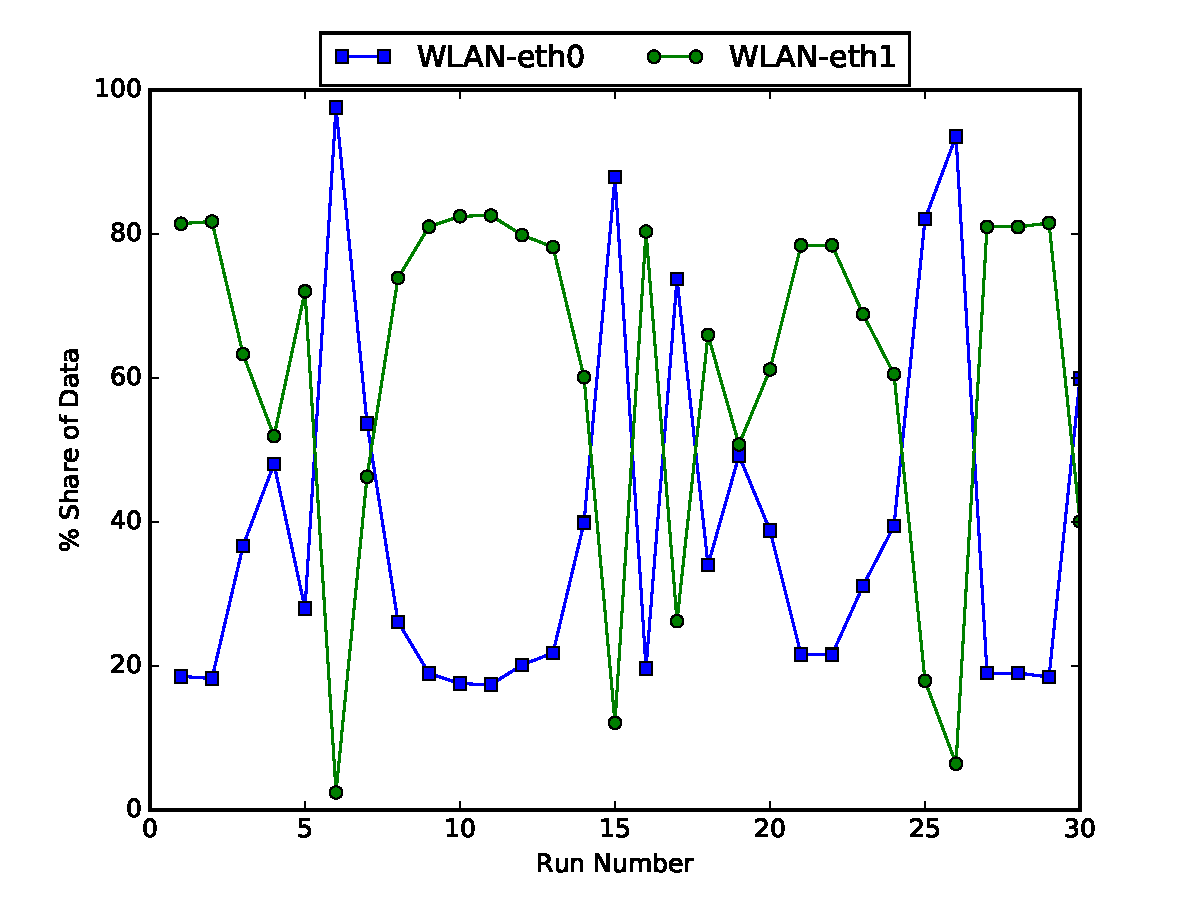
\includegraphics[width=.28\linewidth]{plots/pshare-WLAN-WLAN}
  } &
  \subfloat[3G-3G Scenario packet path split. \label{fig:web:pshare-3g-3g}]
  {
    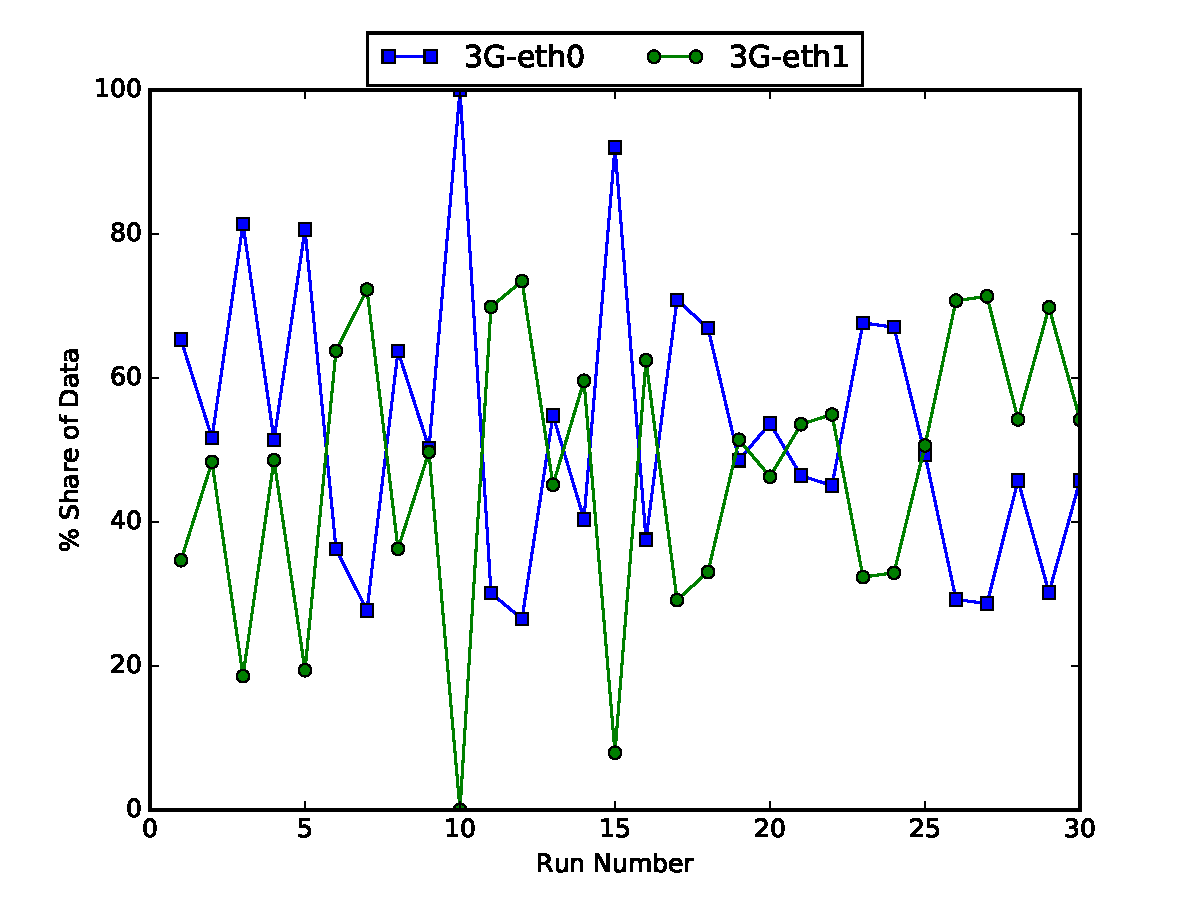
\includegraphics[width=.28\linewidth]{plots/pshare-3G-3G}
  } &
  \subfloat[WLAN-3G Scenario packet path split. \label{fig:web:pshare-wlan-3g}]
  {
    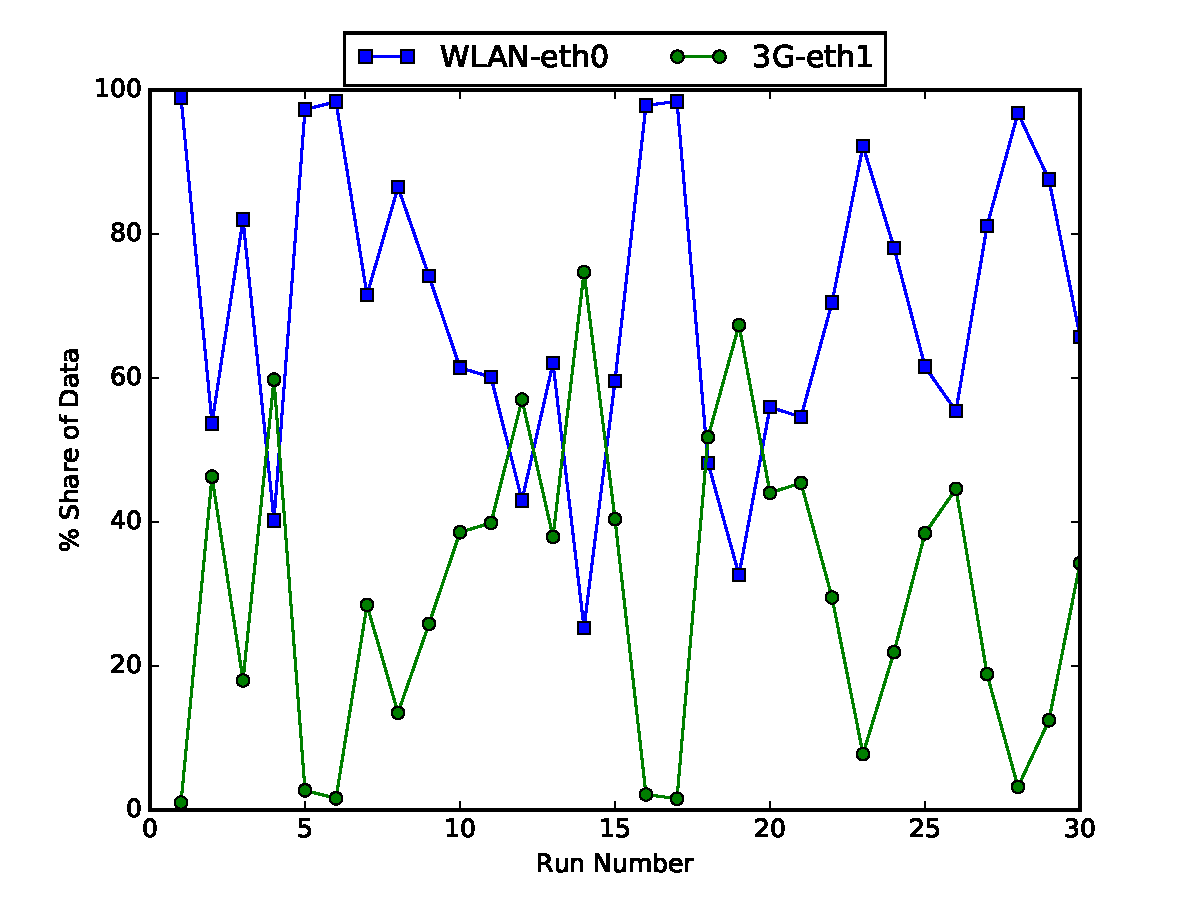
\includegraphics[width=.28\linewidth]{plots/pshare-WLAN-3G}
  }
 \end{tabular}
  \caption{MPTCP percent packets on each path without background traffic}
  \label{fig:web-pshare}
\end{figure*}

\begin{figure*}
  \centering
  \begin{tabular}{ccc}
  \subfloat[WLAN-WLAN Scenario packet path split.\label{fig:web:pshare-wlan-wlan-bg}]{
   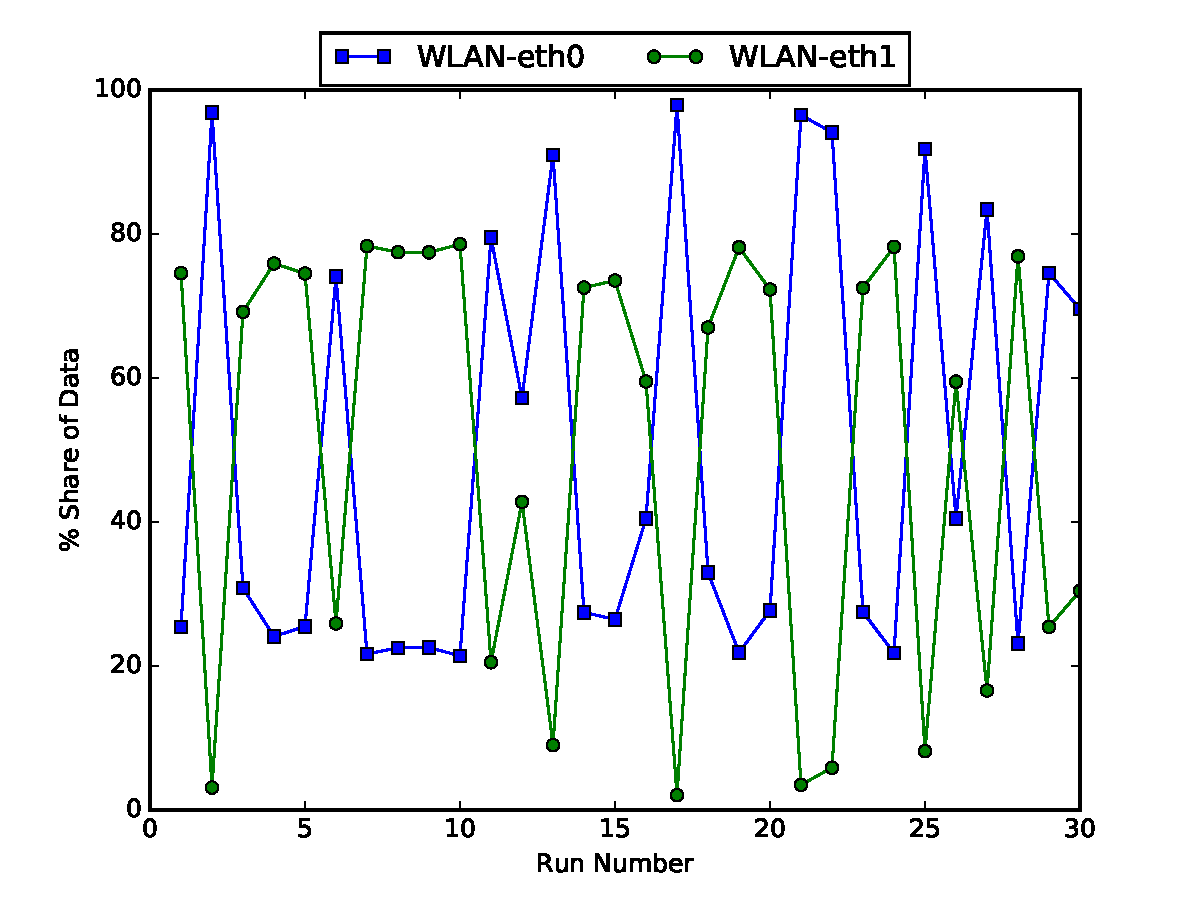
\includegraphics[width=.28\linewidth]{plots/pshare-WLAN-WLAN-BG}
  } &
  \subfloat[3G-3G Scenario packet path split. \label{fig:web:pshare-3g-3g-bg}]
  {
    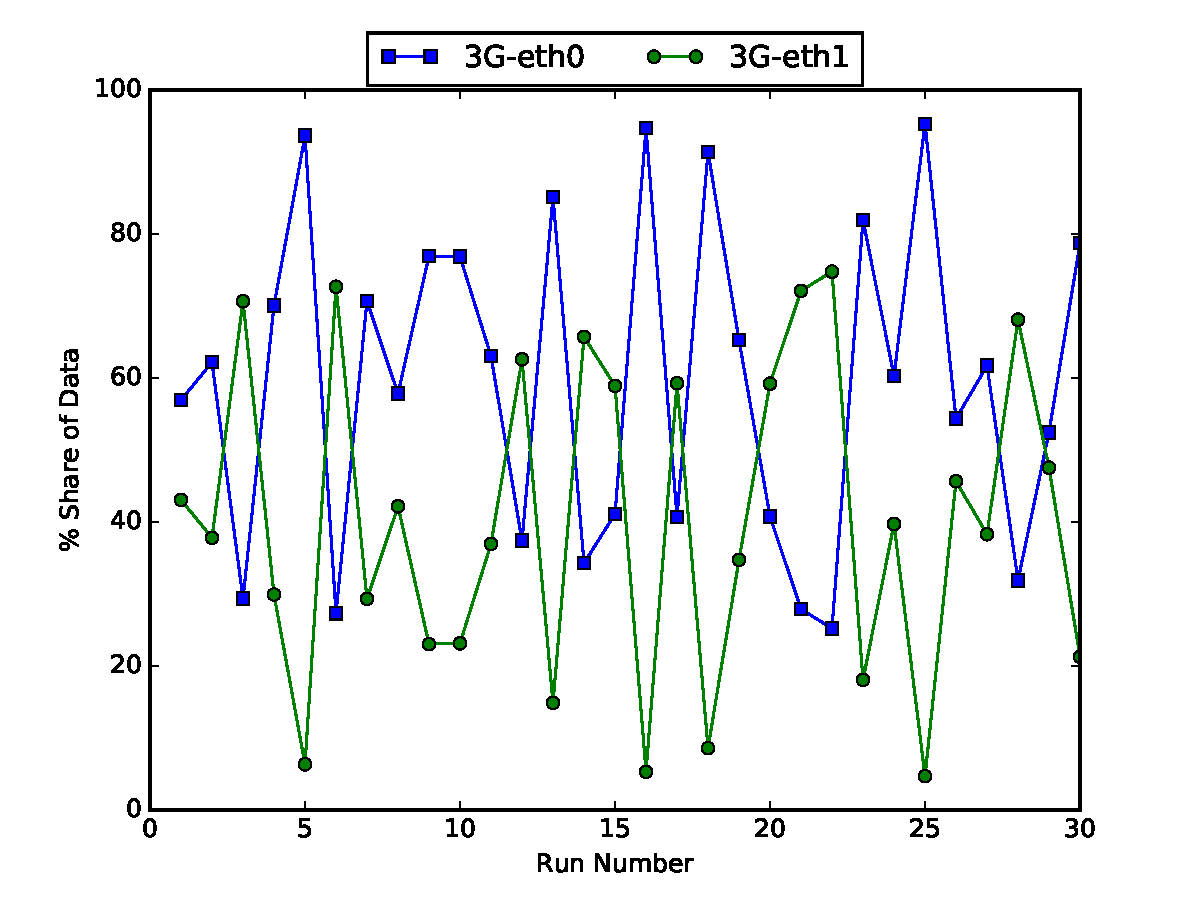
\includegraphics[width=.28\linewidth]{plots/pshare-3G-3G-BG}
  } &
  \subfloat[WLAN-3G Scenario packet path split. \label{fig:web:pshare-wlan-3g-bg}]
  {
    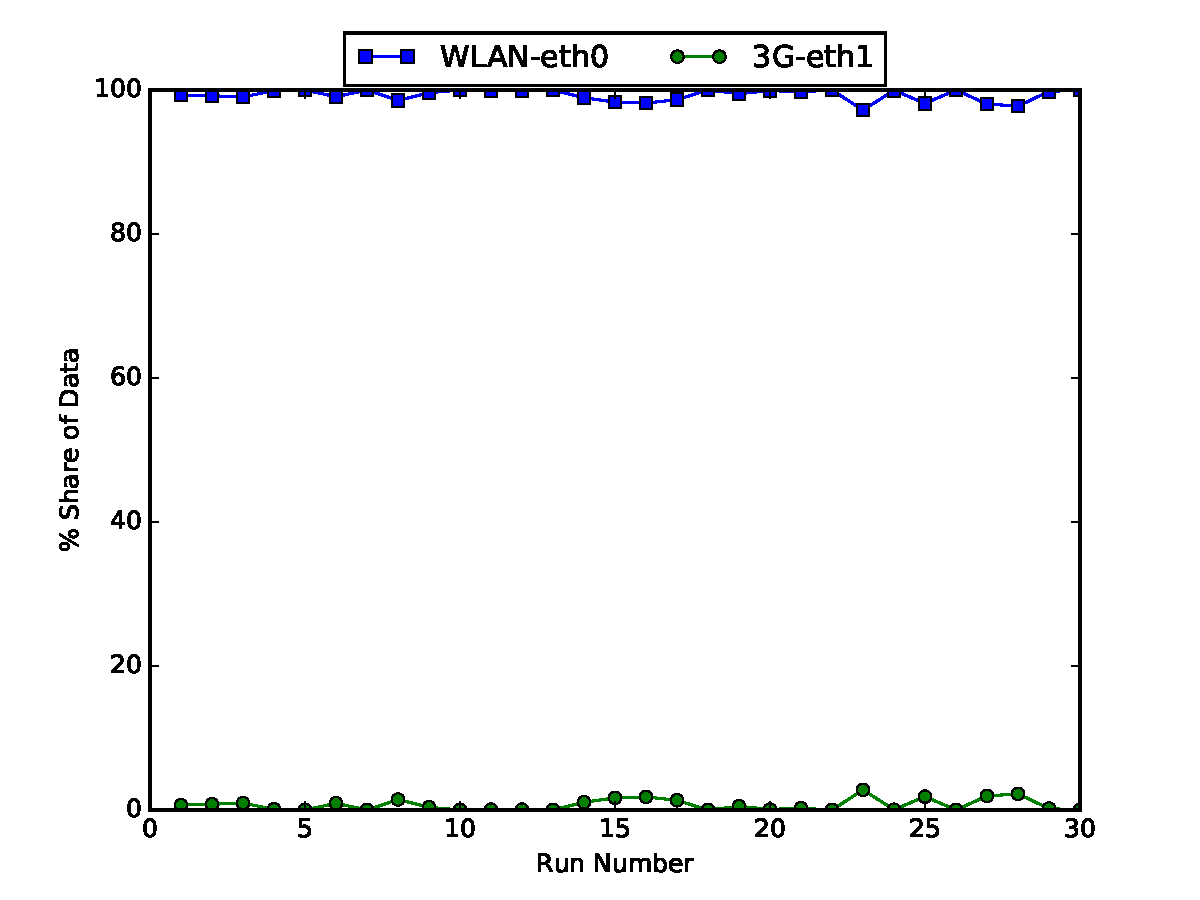
\includegraphics[width=.28\linewidth]{plots/pshare-WLAN-3G-BG}
  }
 \end{tabular}
  \caption{MPTCP percent packets on each path with background traffic}
  \label{fig:web-pshare-bg}
\end{figure*}

For Amazon and Huffpost, we observe similar behavior for no background and with background traffic cases in all the three scenairos. 
As expected, the download times are higher in the background case due to competing flows. 

\begin{figure}[!th]
\begin{minipage}[t]{0.48\textwidth}
\begin{center}
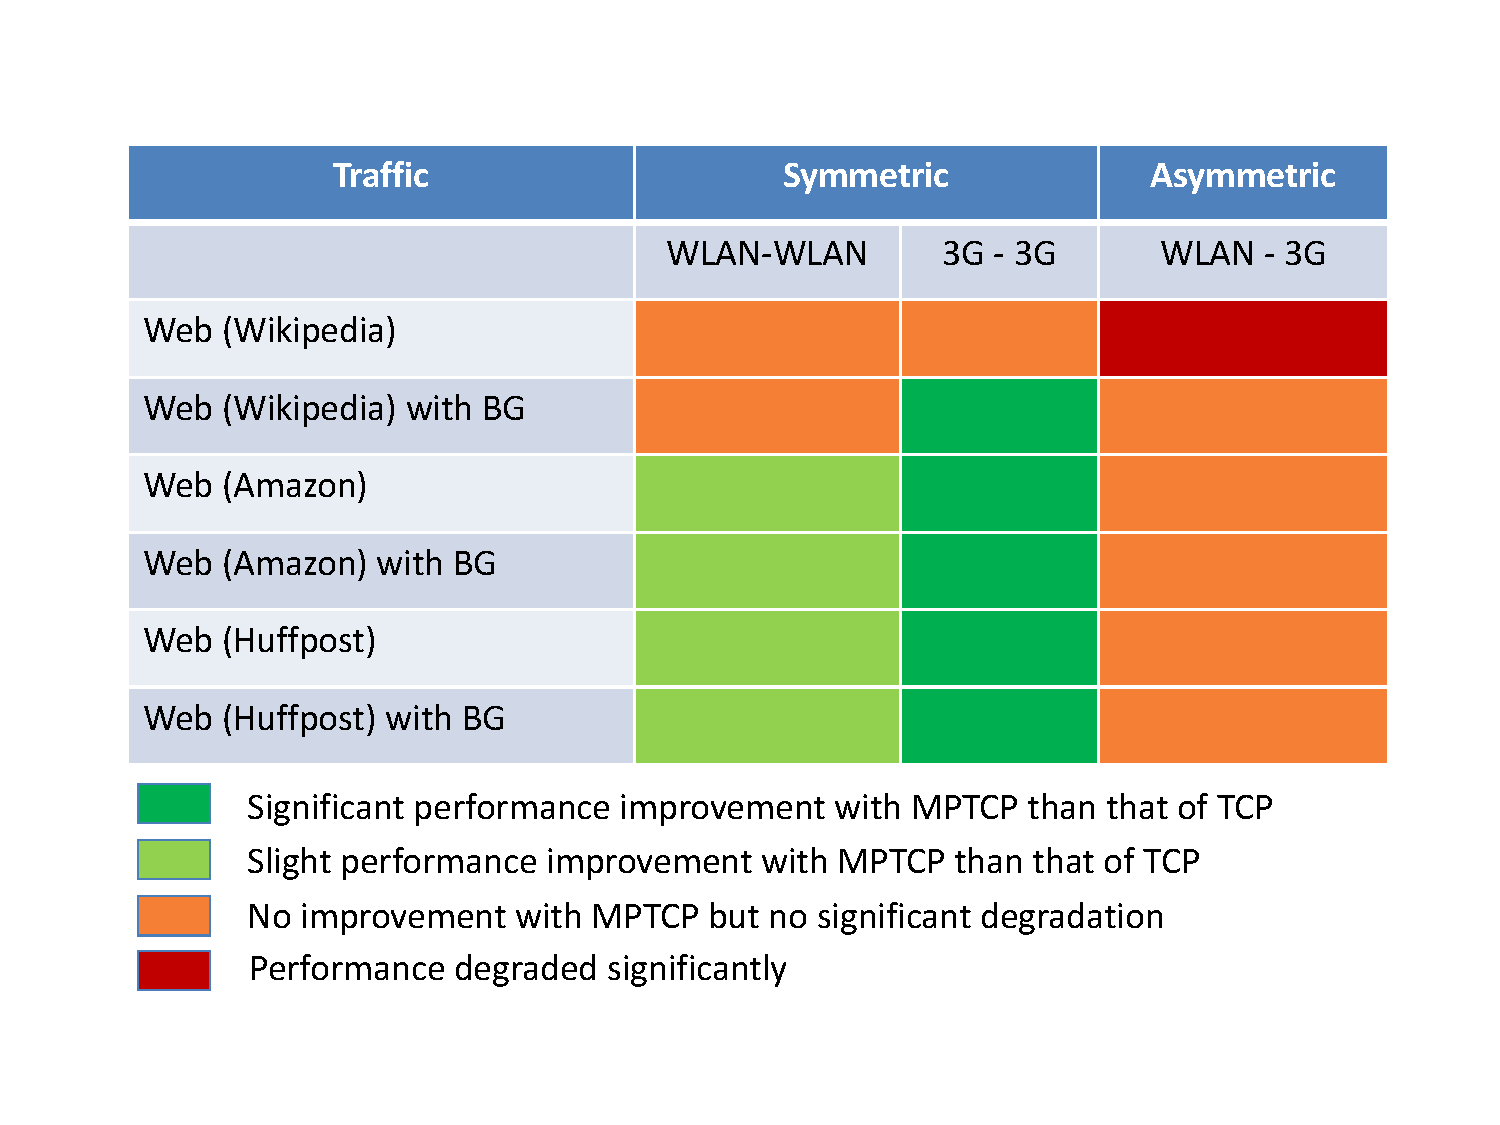
\includegraphics[width=.98\linewidth]{plots/MPTCP-Web}
\end{center}
\caption{Comparison of web traffic latency using MPTCP and TCP}
  \label{fig:web-summary}
\end{minipage}
\end{figure}

Further we analyze the percent share of traffic on each paths for all scenarios. Figures~\ref{fig:web-pshare} and~\ref{fig:web-pshare-bg} reflects the 
share of data downloaded on each interface in no background traffic and with background traffic scenarios respectively. This analysis provides insight
in understanding the improvement or degradation of performance in the operational use of MPTCP in all scenarios. In the case of no background traffic,
the data is split between two paths for all scenarios. This is due to the fact that there is not enough data to transfer compared to the capacity of the
link. The packet scheduler of MPTCP uses the path with lowest RTT in its default setting. WLAN being signficantly faster than 3G, should transfer more share of data in asymmetric sceario. But the considerable split of data usage on 3G is due to the losses in WLAN and some of the flows being extremely
slow to wait for the WLAN RTT estimate recovery after loss.

With background traffic, the percent share of data is similar to that of the no background in symmetric scenarios with significant split between paths.
In asymmetric case, most of the data is transfered on WLAN and very little data is seen in 3G. This is due to multiple reasons including not enough data 
to transfer at WLAN rates making it impossible to switch to 3G, losses in the background flows, and no losses in the foreground flows.

In this paper, we considered different cases to observe the performance of MPTCP in terms of web traffic latency. We believe it is extremely important to
summarize our results in a form of systematic comparison to reduce presentation complexity. In Figure \ref{fig:web-summary} we provide a comparison 
chart of web traffic latency in using MPTCP and TCP across all scenarios. This chart covers all the cases emulated and the corresponding observations where $BG$ signifies with Background traffic. 
